\documentclass[10pt,twocolumn]{article}
\usepackage{graphicx}
\usepackage{amssymb}
\usepackage{titling}
\usepackage{url,hyperref}

\begin{document}

\title{Machine Learning Assignment 2}

\author{Michelle Ho and Shay Lehmann}

\date{%
CUSP-GX-5006\\
Assignment \# 1\\
\rule{\textwidth}{1pt}
}

\posttitle{\par\rule{3in}{0.4pt}\end{center}\vskip 0.5em}
%\postdate{\rule{\textwidth}{1pt}}

\maketitle

\begin{abstract}
In this assignment, the authors explore how New Yorkers seek medical advice and how
this can be predicted by other variables found in the NYC Community Health Survey.
The exercise demonstrates that the use of Naive-Bayes and Support Vector Machine (SVM)
classification techniques and their in performance in a real life scenario.
\end{abstract}

The main goal of this assignment is to demonstrate the use of two classification
techniques, Naive-Bayes and Support Vector Machine (SVM), on predicting how
New Yorkers seek medical advice.

The authors examined the results of the Community Health Survey (CHS) conducted
by the New York City Department of Health and Mental Hygiene. This rich dataset
includes measurements on multiple aspects of health-- including access, nutrition,
demographic information, diet and exercise habits, medical history, and lifestyle
choices.

The motivation is to better understand how New Yorkers seek and receive advice
for their medical needs. Outreach programs hoping to improve access to health care
can make use of these results.

\section{Methods and Data Sets}

The raw dataset of the 2014 NYC Community Health Survey contains 8562 observations
across 188 variables. For this assignment, a subset of the raw dataset was used
for analysis, and the variables are described below:

\begin{itemize}
\item Sick Advice: A categorical variable about the respondent's usual resource for
health advice. This is the dependent variable in the analyses for this
assignment. The options are
"A private doctor",
"Community health center",
"A hospital outpatient clinic",
"ED/ urgent care center",
"Alternative health care provider",
"Family/friend/self/resources",
"Non-hospital clinic",
"Other",
"No usual place", or
"Clinic, unknown type".
\item Education: A categorical variable on educational attainment. Categories are "Less than HS", "High school grad",
"Some college", or "College graduate"
\item Marital status: A categorical variable on marital status. Categories are
"Married",
"Divorced",
"Widowed",
"Separated",
"Never married", or
"Member of unmarried couple living together"
\item US born: A binary variable answering the yes or no question "Are you US or foreign born?"
\item Sexual ID: A categorical variable on sexual orientation. Categories are
"Heterosexual",
"Gay/Lesbian", or
"Bisexual"
\item At Home Language: A categorical variable answering the question "What language do you
speak most often at
home?" Options are
"English",
"Spanish",
"Russian",
"Chinese",
"Indian", or
"Other"
\item Insured: A binary variable answering the yes or no question "Do you have any
kind of health
insurance coverage,
including private
health insurance,
prepaid plans such as
H-M-Os, or
government plans
such as Medicare or
Medicaid?"
\item The dependent variable being predicted is 'Sick Advice' in this assignment's
analyses. The authors refer to this variable as 'Y'.
\item The independent variables are all the others.
\item  For all variables, the options "do not know" and "refuse"
were treated as null values and dropped.
\end{itemize}


The steps taken for this assignment:

\begin{enumerate}
\item First, an ordinary least squares linear regression model was fitted for
the normalized, raw dataset (LM1).
\item Then, the dataset was projected into its principal components and the linear
regression was re-run with all principal components (LM2).
\item The linear regression was re-run with the first three principal components (LM3).
\item The LM1 and LM3 linear models are assessed with cross validation.
\item An ordinary least squares linear regression model was fitted for the
raw dataset with the categorical variables (BldClassif and Neighborhood) removed (LM4).
\item This new linear regression model is assessed with cross validation.
\item Finally, lasso and ridge regression are performed on the raw dataset
with categorical variables removed.
\end{enumerate}


\section{Results}

The first linear model generated was fitted for normalized, raw data with all dependent
variables.  The second linear model was fitted after projecting the data onto
five principal components. The coefficients for these models are reported in
Table 1. The x1, x2, x3, x4 and x5 coefficients have no interpretable
meaning. The 'Neighborhood' and 'BldClassif' variables also have little
interpretable value, since they are being treated as non-categorical at this point.
Both models have the same Mean Square Error (MSE), as expected because I kept
all five principal components, which can be thought of as a rotation of
the "coordinate system" of our raw data. The MSE for both is about 0.02705.

The R-squared value for both models is very low (0.001), and every variable or component's
p-value is above 0.08, indicating that these models are very poor. It's possible that
these variables or components are zero or even the opposite sign. The plot of
actual Y versus predicted Y for LM1 (Figure 1) shows that the model is predicting
very close to 0.41 for almost all inputs, which is in fact the mean market value
per square foot (without normalization, this is \$128.75/square foot). In other words,
this model is not very sophisticated and is only predicting the mean.

Next, I keep only the first three principal components. I chose the first
three via the "elbow" method, where there appears to be a slight inflection point
in the explained variance ratio (Figure 2). By incrementally increasing the number
of principal components, I find that the mean square error approaches the mean
square error of the regular linear model and that the percentage of explain variances
approaches 100\%. With three principal components, approximately 81\% of the
variance in the data is preserved.

In using PCA to project our raw data and then only selecting the first three
principle components to fit the linear model, I am hoping to reduce the
"noise" inside the data. This third linear model shows little improvement
on the first two linear models. The R-squared is even lower, 0.0002, and three components
have high p-values. The plot of actual vs predicted (Figure 3) shows even less sophistication.
Remember, though, that I have not removed outliers and that PCA can be influenced by outliers
pulling the components toward unhelpful directions. Furthermore, PCA-featured
linear regression with fewer components than original variables always performs
worse because there is a loss of information. The main goal is to reduce covariances,
reduce dimensionality, and create a smoother model. In this situation, with so few
independent variables to begin with, the loss of information may be doing
more harm than good.

Nonetheless, I assess the performance of this PCA-featured linear model (LM3)
and the first linear model (LM1) via cross validation for comparison.
The data is split 33\% to testing and the rest to training. To assess the
first method, a linear model is fit on the training data and in-sample R-squared
is calculated. The fitted model is then used to predict the test data set, and
the out-of-sample R-squared is calculated. Repeated 1000 times, this yields an
in-sample R-squared of 0.0021 and out-of-sample R-squared of -0.0054.

Cross validation is also applied to the PCA-featured linear model (LM3). PCA is used
only on the training set to find the principal components. The linear regression model
is fit for these components. Then, the test data is projected onto the first three
components, and the model predicts on the transformed test data. Repeated 1000 times,
this yields an average in-sample R-squared of 0.00094 and out-of-sample R-squared of
-0.00376.

It appears that the out-of-sample R-squared terms for both the PCA-featured and non-PCA featured linear models
are both negative. The only way to achieve a negative R-squared is to have the
predicted values error be worse than the error from simply predicting the mean.
However, it is interesting to note that the in-sample R-squared for the
LM1 model is slightly higher than the in-sample R-squared of the LM3 model,
yet the out-of-sample R-squared of LM1 is slightly lower than LM3's. This may indicate that our
PCA-featured linear model does a bit better out of sample, but not by much.

I repeat the steps for linear regression after removing the categorical variables 'Neighborhood'
and 'BldClassif'. The results are reported in Table 4. Cross validation is also applied to this
new model, and the average in-sample R-squared after 1000 repetitions is 0.0017
Out of Sample R-squared for 1000 times is -0.0035. Again, the model appears to be
very poor, but there is slight improvement in the out-of-sample R-squared.

Finally, ridge and lasso regression models are also fitted using the non-categorical data. Figure
4 shows the predicted versus actual outcome of the L4 model (red), ridge regression model
(green) and lasso regression model (black). Like the reduced dimension PCA-featured
linear regression, these two shrinkage models also show the predicted values
become simpler and smoother. Figure 5 shows the change in MSE as alpha, the regularization term,
increases. Figure 6 shows how the coefficients shrink to zero as alpha increases.

\section{Conclusions}

In summary, the models generated for this assignment failed at predicting
the market value per square foot of a Manhattan building based on a handful of
explanatory variables. Efforts to improve a simple linear model with PCA dimension reduction,
and shrinkage methods with lasso and ridge regression did not improve model performance.
There are several reasons that account for the poor performance. First, with only
5 explanatory variables, there is more harm done in reducing information or dimensionality than
there is gained in "smoothing" the model. Second, outliers were not removed in
the dataset, which may have altered how the principal components were calculated.
Finally, ~2000 observations may not have been enough to represent the very diverse
building landscape of Manhattan.

Python code used to generate the results, tables, and figures for this assignment can be
found at \url{https://github.com/michellemho/machine_learning_for_cities}.

\begin{center}
\begin{table*}[]
\centering
\caption{Results of Linear Models with Raw Normalized Data}
\label{my-label}
\begin{tabular}{lllll}
                & Normalized raw data (LM1) &          & PCA-featured data (LM2) & \\
constant        & 0.40926343                & constant & 0.4101                  & \\
Neighborhood    & -0.12254491               & x1       & -0.0379                 & \\
BldClassif      & 0.02690248                & x2       & -0.0113                 & \\
YearBuilt       & 0.02695934                & x3       & -0.0441                 & \\
GrossSqFt       & 0.13819696                & x4       & -0.1773                 & \\
GrossIncomeSqFt & 0.01101943                & x5       & -0.0273                 & \\
R-squared       & 0.001                     & R-squared& 0.001                   & \\
                &                           &          &                         &
\end{tabular}
\end{table*}
\end{center}

\begin{table*}[]
\centering
\caption{Results of Linear Model on Non-Categorical Data}
\label{my-label}
\begin{tabular}{lll}
                & LM4        &  \\
constant        & 0.4101     &  \\
YearBuilt       & -0.0626    &  \\
GrossSqFt       & 0.1038     &  \\
GrossIncomeSqFt & -0.1151 &  \\
R-Squared       & 0.001     &
\end{tabular}
\end{table*}

\begin{figure*}[]
  \begin{center}
    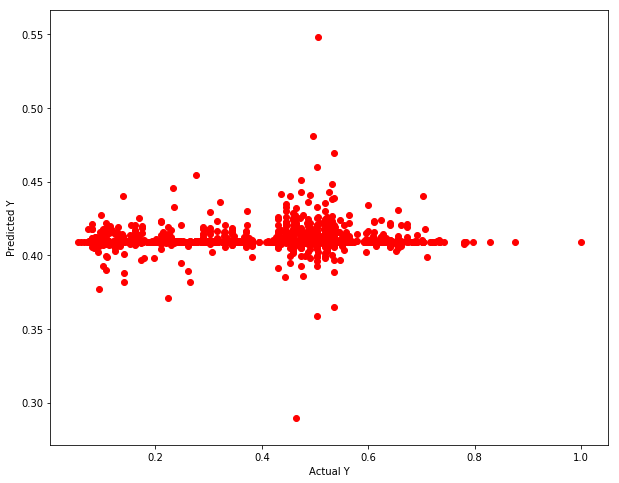
\includegraphics[width=2.5in]{figure1.png}
  \end{center}

  \caption{\small Actual vs Predicted -- Linear Model LM1}
  \label{fig-1}
\end{figure*}

\begin{figure*}[!t]
  \begin{center}
    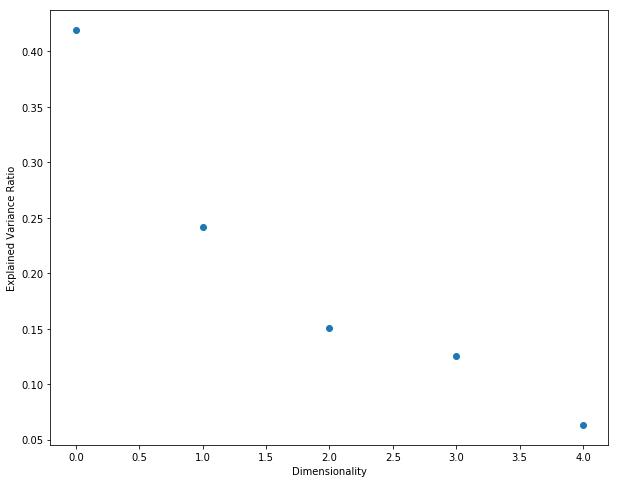
\includegraphics[width=2.5in]{figure2.png}
  \end{center}

  \caption{\small Explained Variance Ratio of Principal Components}
  \label{fig-2}
\end{figure*}

\begin{figure*}[!t]
  \begin{center}
    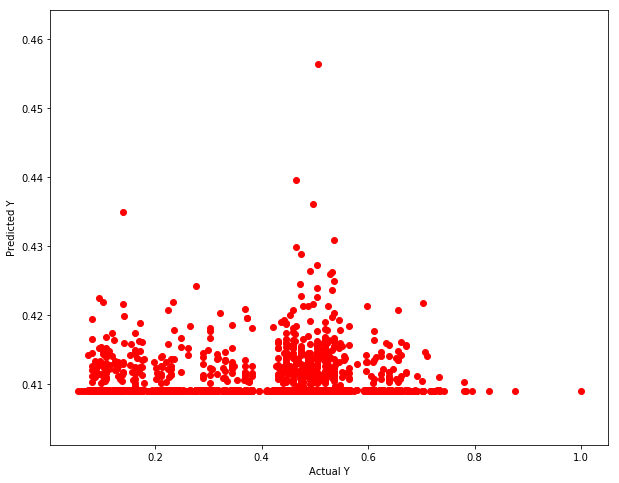
\includegraphics[width=2.5in]{figure3.png}
  \end{center}

  \caption{\small Actual vs Predicted -- PCA-featured Linear Model LM2}
  \label{fig-3}
\end{figure*}

\begin{figure*}[!t]
  \begin{center}
    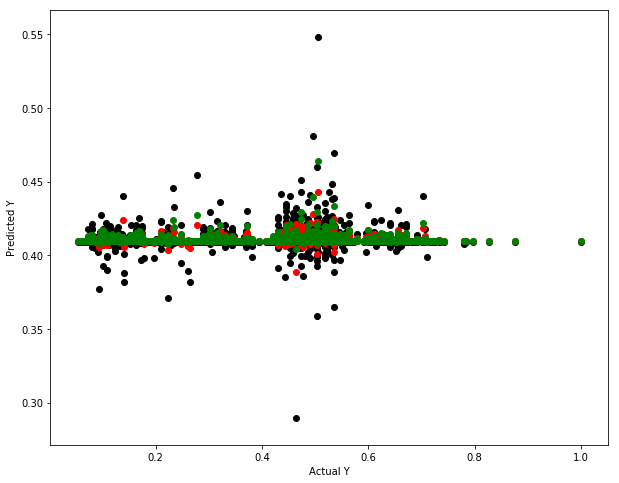
\includegraphics[width=2.5in]{figure4.png}
  \end{center}

  \caption{\small Actual vs Predicted -- L4 model (red), ridge regression model
  (green) and lasso regression model (black)}
  \label{fig-4}
\end{figure*}

\begin{figure*}[!t]
  \begin{center}
    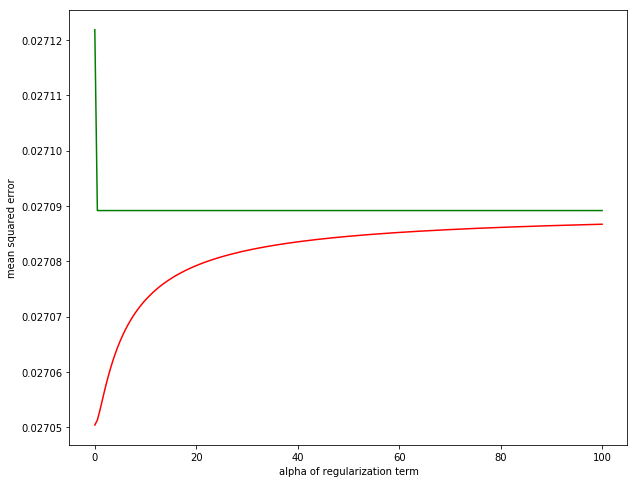
\includegraphics[width=2.5in]{figure5.png}
  \end{center}

  \caption{\small MSE for Ridge and Lasso, increasing alpha}
  \label{fig-5}
\end{figure*}

\begin{figure*}[!t]
  \begin{center}
    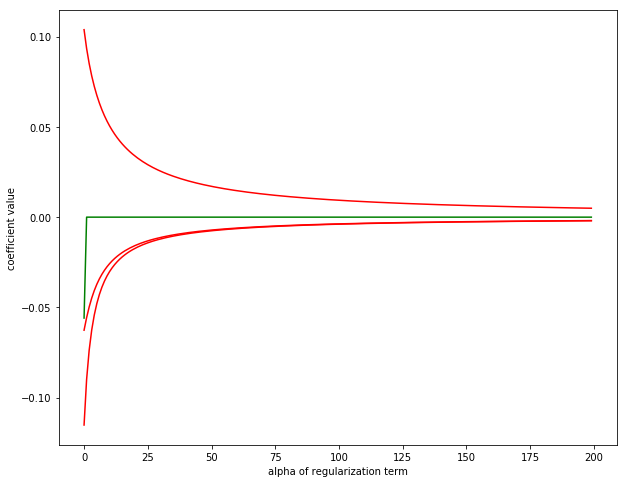
\includegraphics[width=2.5in]{figure6.png}
  \end{center}

  \caption{\small Coefficients for Ridge and Lasso, increasing alpha}
  \label{fig-6}
\end{figure*}



\end{document}
